\section{User Interface in Flutter}\label{sec:flutter-user-interface}
"Flutter includes a modern react-style framework, a 2D rendering engine, ready-made widgets, and development tools.
These components work together to help you design, build, test, and debug apps.
Everything is organized around a few core principles."~\cite{flutterTechnicalOverview}
Flutter has a widget tree that renders widget into a nested tree, and these widgets are covering themselves.
It does not matter if a widget from the widget tree is:
\begin{itemize}
    \item Container,
    \item List View,
    \item Image,
    \item Text,
    \item Animation,
    \item or anything else.
\end{itemize}
A widget or its descendants represent everything in the user interface in Flutter.
Additional important classes for user interface are MaterialApp and Scaffold.~\cite{flutterBook}
MaterialApp and Scaffold, it will be described in the Material Design section~\ref{sec:android-specific-ui-widgets}.

\begin{figure}
    \centering
    \begin{minipage}{.4\textwidth}
        \centering
        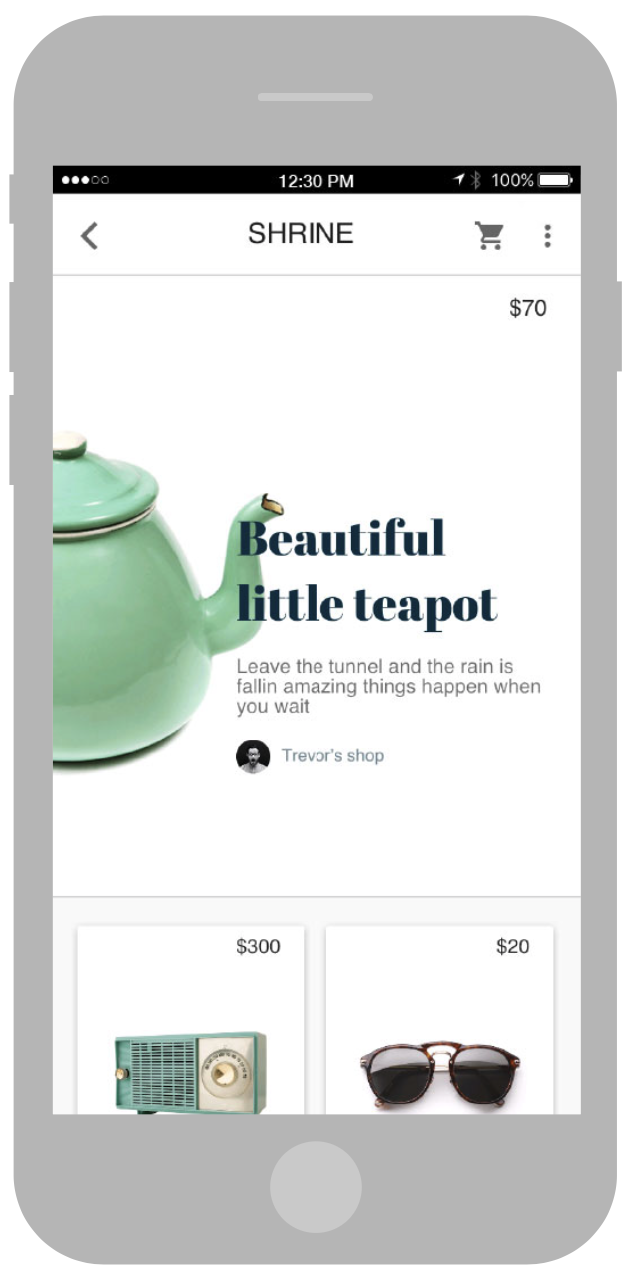
\includegraphics[width=.7\linewidth]{assets/hero-shrine-ios.png}
        \caption{Flutter demo app on iOS~\cite{flutterTechnicalOverview}}
        \label{fig:flutter-demo-app-ios}
    \end{minipage}%
    \hspace{.05\linewidth}
    \begin{minipage}{.4\textwidth}
        \centering
        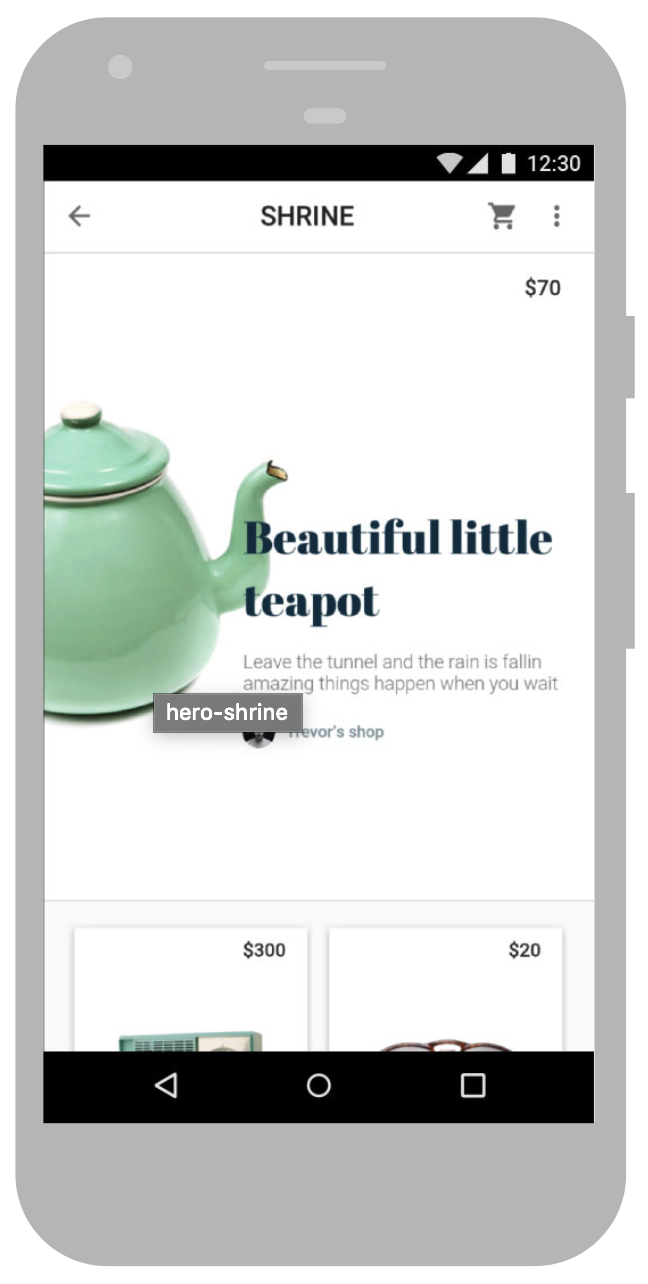
\includegraphics[width=.72\linewidth]{assets/hero-shrine-android.png}
        \caption{Flutter demo app on Android~\cite{flutterTechnicalOverview}}
        \label{fig:flutter-demo-app-android}
    \end{minipage}
    \label{fig:flutter-demo-app}
\end{figure}
